\documentclass[journal]{IEEEtran}
\usepackage[a5paper, margin=10mm, onecolumn]{geometry}
\usepackage{lmodern}
\usepackage{amsmath, amssymb}
\usepackage{graphicx}
\usepackage{hyperref}

\title{8.2.2}
\author{EE24BTECH11004 - Ankit Jainar}
\date{}

\begin{document}

\maketitle

\textbf{Question:}
Find the area bounded by the curves:
\begin{align*}
    (x - 1)^2 + y^2 = 1 \quad \text{and} \quad x^2 + y^2 = 1
\end{align*}

\textbf{Solution:}
\newline
\textbf{Theoretical Solution:}
\newline
The curves are two circles:
\begin{itemize}
    \item Circle 1: $(x - 1)^2 + y^2 = 1$, centered at $(1, 0)$ with radius $1$.
    \item Circle 2: $x^2 + y^2 = 1$, centered at $(0, 0)$ with radius $1$.
\end{itemize}

To find the area of the region bounded by these curves, we determine the points of intersection by solving:
\begin{align*}
    (x - 1)^2 + y^2 &= x^2 + y^2 \\
    \Rightarrow x^2 - 2x + 1 + y^2 &= x^2 + y^2 \\
    \Rightarrow -2x + 1 &= 0 \quad \implies \quad x = \frac{1}{2}
\end{align*}
The points of intersection are $\left(\frac{1}{2}, \frac{\sqrt{3}}{2}\right)$ and $\left(\frac{1}{2}, -\frac{\sqrt{3}}{2}\right)$.

The area between the curves is computed by subtracting the integrals of the two curves in the interval where they overlap.
\newline
\textbf{Computational Solution (Trapezoidal Rule):}
\newline
Using the trapezoidal rule to approximate the area, we write:
\begin{align*}
    A \approx \int_{x_1}^{x_2} \left[ f(x) - g(x) \right] dx
\end{align*}
Here, $f(x)$ and $g(x)$ represent the upper and lower curves, respectively, and $[x_1, x_2]$ is the interval of integration.

Divide the interval into $n$ subintervals of width $h = \frac{x_2 - x_1}{n}$. The trapezoidal rule states:
\begin{align*}
    A \approx \frac{h}{2} \left[ (f(x_1) - g(x_1)) + 2\sum_{i=1}^{n-1} (f(x_i) - g(x_i)) + (f(x_n) - g(x_n)) \right]
\end{align*}
\newline
Substituting the functions:
\begin{align*}
    f(x) = \sqrt{1 - (x - 1)^2}, \quad g(x) = \sqrt{1 - x^2}
\end{align*}
\newline
Calculate $x_i$, $f(x_i)$, and $g(x_i)$ at each step $i$:
\begin{align*}
    x_i &= x_1 + i \cdot h, \quad f(x_i) = \sqrt{1 - (x_i - 1)^2}, \quad g(x_i) = \sqrt{1 - x_i^2}
\end{align*}
\newline
By iterating over $n$ intervals, approximate the area. A comparison of the theoretical and computational results is shown below.
\newline
\textbf{Comparison of Results:}
\begin{figure}[h!]
    \centering
    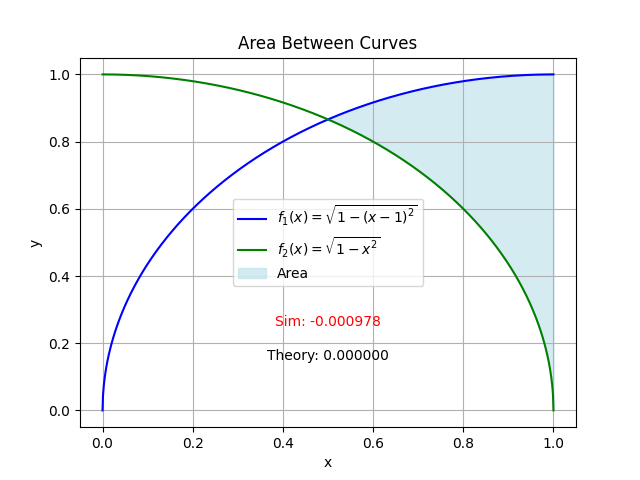
\includegraphics[width=\columnwidth]{figs/fig.png}
    
\end{figure}

\end{document}

